\chapter{Creating Custom Metrics}\label{ch:custom_metrics}

\section{Conceptual Overview} 

\begin{figure}[h]
	\centering
	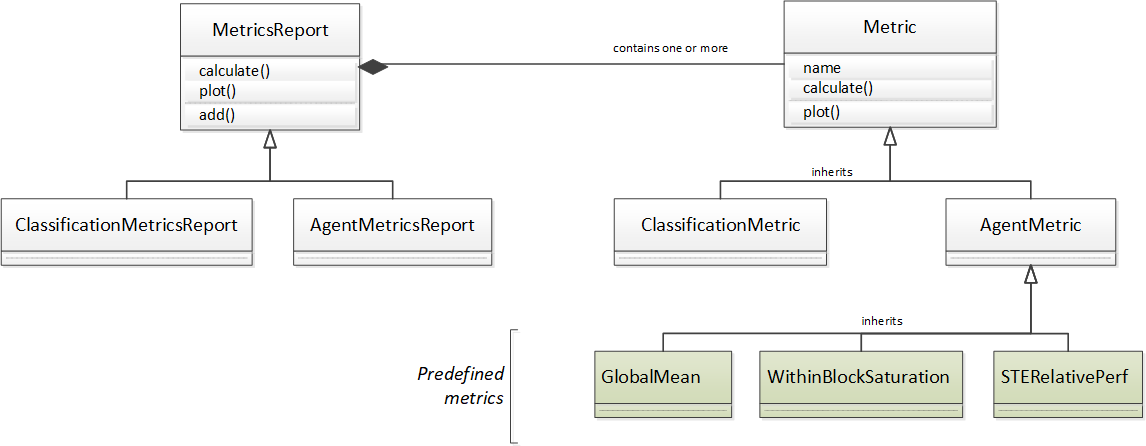
\includegraphics[width=1\columnwidth]{sections/figs/metrics_framework_uml.png}
	\caption{UML Diagram for classes in the Metrics Framework. The predefined metrics\\shown are a subset of the full set of metrics, and shown only for illustration.}
	\label{fig:umlframework}
\end{figure}

Conceptually, a MetricsReport object contains one or more Metrics. By default, this includes a set of predefined Metrics (such as GlobalMean or WithinBlockSaturation). The MetricsReport.calculate() method loads the log data into a Pandas dataframe, does some pre-processing and cleanup, and then hands the dataframe to each Metric’s calculate() method. Figure~\ref{fig:umlframework} shows the diagram for the classes in the Metrics Framework (specifically, the l2metrics Python package).\\[0.2in]

Consequently, it is easy to author and use a custom Metric, as follows:\\[0.1in]
    1. Create a Python class, subclassing from the ClassificationMetric or AgentMetric as appropriate\\
    2. Implement the interface (in particular, the name property and calculate() method)\\
    3. Write a top-level script that instantiates the ClassificationMetricsReport or AgentMetricsReport (as appropriate) and adds the custom metric to the report (replacing or augmenting the predefined metrics).\\
    4. Run the top-level script.\\[0.1in]
\iffalse
\section{Sample Workflow}

In \verb|l2metrics/core.py| we introduce an abstract Metric class which describes the general format for any Metric you may use or write, whether for Agent or Classification Learners. The core content of each Metric is contained in the calculate method, which has the following required arguments: the log data, a phase\_info dataframe, and a metrics\_dict dataframe. The metrics\_dict starts blank and is filled by each metric in its turn, whereas the log data and the phase info are extracted in the MetricsReport constructor from the logs via two helper functions: \\[0.1in]

l2metrics/util.py - (read\_log\_data): scrapes the logs and returns a pandas dataframe of the logs and task parameters\\
l2metrics/\_localutil.py - (parse\_blocks): builds a pandas dataframe of the phase information contained in the log data\\[0.1in]

These dataframes are passed along by the MetricsReport to the appropriate metric and thus the Metrics and MetricsReport classes should be utilized in conjuction with each other. Though there are a list of default metrics which the MetricsReport uses for the Core Capabilties being exercised at this time, you may choose to add your own metric to this list by using the add method on MetricsReport. 

Please see the calc\_metrics.py file for an example on how to get started with writing your own custom metric. A simple whole-dataframe-mean is currently implemented as an example to help get you started.

\begin{verbatim}    

def calculate(self, dataframe, phase_info, metrics_dict):
        return {'global_perf': dataframe.loc[:, "reward"].mean()}, {'global_perf': dataframe.loc[:, "reward"].mean()}
\end{verbatim}

\fi
